\documentclass[a4paper]{article}
\usepackage[T2A]{fontenc}
\usepackage[utf8]{inputenc}
\usepackage[ukrainian]{babel}
\usepackage{tikz}
\usepackage{lastpage} 
\usepackage[left=2.5cm, right=1.5cm, top=1.5cm, bottom=2.7cm]{geometry}
\usepackage{fancyhdr}
\usepackage{amsmath, amssymb, amstext} % Математичні символи
\usepackage{fp}
\usepackage{ragged2e}

\usepackage{listings}

\usepackage{xifthen} % Для умовних перевірок

% \usepackage{fontspec}
% \setmainfont{Times New Roman}

\usepackage{caption}


% \usepackage{graphicx}

\pagestyle{fancy}
\fancyhf{}
\renewcommand{\headrulewidth}{0pt}
\renewcommand{\footrulewidth}{0pt}

% \pagestyle{empty}

\newcommand{\makrosCalc}[1]{
    \FPeval{\the\fpresult}{#1}
}

\newcommand{\makrosmytitle}[2]{
    \thispagestyle{empty}
    \centering
    \textbf{Міністерство освіти і науки України}\\
    \textbf{КИЇВСЬКИЙ ПОЛІТЕХНІЧНИЙ УНІВЕРССИТЕТ}\\[2cm]
    \raggedleft
    Кафедра автоматизації та систем неруйнівного контролю\\
    Група ПМ-11
    \vfill
    \centering
    \textbf{ПРОЕКТУВАННЯ СИСТЕМ АВТОМАТИЗАЦІЇ}\\[1cm]
    \textbf{ЗВІТ З #1}\\[1cm]
    \textbf{\huge #2}
    \vfill
    \begin{flushleft}
        Керівник  \qquad\qquad\quad \hfill\qquad (підпис)\hfill 
        д.т.н., проф. Черепанська І. Ю.\\
        \hfill (дата)\\[2cm]
        Виконавець\hfill (підпис)\hfill Юша Володимир Ігорович\\
        \hfill (дата)
    \end{flushleft}
    \vfill
    \centering
    2025
}

\newcommand{\makrosFrameBig}[2]{
    \thispagestyle{empty} % Вимикає номер сторінки на першій сторінці
    
    \begin{tikzpicture}[remember picture, overlay]
        \begin{scope}[shift={([xshift = 20 mm, yshift = 10 mm]current page.south west)}]
            \draw[line width=2] (0,0) rectangle (180 mm,277 mm);
        \end{scope}
    \end{tikzpicture}
    
    \begin{tikzpicture}[remember picture, overlay]
        \begin{scope}[shift={([xshift = 20 mm, yshift = 10 mm]current page.south west)}, x=1mm, y=1mm]
            \draw[line width=2] (0,0) rectangle (180,40);
            \draw[line width=2]  (7,40) -- (7, 25);
            \draw[line width=2] (17,40) -- (17, 0);
            \draw[line width=2] (40,40) -- (40, 0);
            \draw[line width=2] (55,40) -- (55, 0);
            \draw[line width=2] (65,40) -- (65, 0);
            \draw[line width=2] (135,25) -- (135,0);
            \draw[line width=2] (140,15) -- (140,20);
            \draw[line width=2] (145,15) -- (145,20);
            \draw[line width=2] (150,25) -- (150,15);
            \draw[line width=2] (165,25) -- (165,15);
        
            \draw (0,35) -- (65, 35);
            \draw[line width=2] (0,30) -- (65, 30);
            \draw[line width=2] (0,25) -- (180, 25);
            \draw (0,20) -- (65, 20);
            \draw (0,15) -- (65, 15);
            \draw (0,10) -- (65, 10);
            \draw (0,5) -- (65, 5);
        
            \draw[line width=2] (135,20) -- (180, 20);
            \draw[line width=2] (135,15) -- (180, 15);
            
            \node at (3.5, 27.5) {Зм.};
            \node at (12, 27.5) {Лист};
            \node at (28.5, 27.5) {№ докум.};
            \node at (47.5, 27.5) {Підпис};
            \node at (60, 27.5) {Дата};
            
            \node at (7, 22.5) {Розроб.};
            \node at (6.5, 17.5) {Перев.};
            \node at (8.5, 7.5) {Н. Контр.};
            \node[align=left] at (5, 2.5) {Затв.};
            
            \node at (142.5, 22.5) {Літ.};
            \node at (157.5, 22.5) {Аркуш};
            \node at (172, 22.5) {Аркушів};
        
            \node[align=left, font=\itshape, anchor=south west, scale=0.9] at (16, 20) {Юша В. І.};
            \node[align=left, font=\itshape, anchor=south west, scale=0.8] at (16, 15) {Черепанська І.Ю.};
            \node[align=left, font=\itshape, anchor=south west, scale=0.8] at (16, 0) {Черепанська І.Ю.};
        
            \node[anchor=center, font=\itshape, scale=1.5] at (122, 32) {#1};
            \node[align=center, font=\itshape, anchor=center] at (100, 12) {#2};
            \node[align=left, font=\itshape, anchor=south west, scale=0.9] at (135, 5) {КПІ ім. І. Сікорського, ПБФ};
            \node[anchor=center, font=\itshape] at (158, 17) {2};
            \node[anchor=center, font=\itshape] at (172, 17) {\pageref{LastPage}};    
        \end{scope} 
    \end{tikzpicture}
}

\newcommand{\makrosFrameSmall}[1]{
    % \thispagestyle{empty} % Вимикає номер сторінки на першій сторінці
    
    \begin{tikzpicture}[remember picture, overlay]
        \begin{scope}[shift={([xshift = 20 mm, yshift = 10 mm]current page.south west)}]
            \draw[line width=2] (0,0) rectangle (180 mm,277 mm);
        \end{scope}
    \end{tikzpicture}
    
    \begin{tikzpicture}[remember picture, overlay]
        \begin{scope}[shift={([xshift = 20 mm, yshift = 10 mm]current page.south west)}, x=1mm, y=1mm]
            \draw[line width=2] (0,0) rectangle (180,15);
            \draw[line width=2] (7,0) -- (7, 15);
            \draw[line width=2] (17,0) rectangle (43,15);
            \draw[line width=2] (55,0) rectangle (64,15);
            \draw[line width=2] (170,0) -- (170, 15);

            \draw[line width=2] (0,5) -- (64, 5);
            \draw               (0,10) -- (64, 10);
            \draw[line width=2] (170,8) -- (180, 8);

            \node[anchor=center, scale=0.8] at (3.5, 2.5) {Змн.};
            \node[anchor=center, scale=0.9] at (12, 2.5) {Арк.};
            \node[anchor=center] at (30, 2.5) {№~докум.};
            \node[anchor=center, scale=0.9] at (49, 2.5) {Підпис};
            \node[anchor=center, scale=0.9] at (59, 2.5) {Дата};
            \node[anchor=center, font=\itshape, scale=1.5] at (115, 7.5) 
                {#1};
            \node[anchor=center] at (175, 12) {Арк.};
            \node[anchor=center] at (175, 4) {\thepage};
            
        \end{scope}
    \end{tikzpicture}
}

% % \makrosLab{1}{Шифр}{Назва}
% \newcommand{\makrosLab}[3]{ 
%     \fancyfoot[C]{\makrosFrameSmall{#2}}
%     \ifthenelse{\equal{#2}{л}}%    
%     % \makrosmytitle{#1}{#3}
%     \newpage
%     \makrosFrameBig{#2}{#3}
%     \justify
%     \fontsize{14}{16}\selectfont
%     \section*{Лабораторна робота №#1}
% }

% Оголошуємо змінні
\newcommand{\mytitlegenitive}{}
\newcommand{\mytitle}{}
\newcommand{\shyfr}{}

% \makrosLab{номер}{п чи л}{Назва}
\newcommand{\makrosLab}[3]{ 


    % Перевіряємо другий аргумент
    \ifthenelse{\equal{#2}{л}}%
        {
            \renewcommand{\mytitle}{Лабораторна робота №#1}
            \renewcommand{\mytitlegenitive}{ЛАБОРАТОРНОЇ РОБОТИ №#1}
            \renewcommand{\shyfr}{ПМ1115.04.00.0#1 ЛР}
        }%
        { \ifthenelse{\equal{#2}{п}}%
            {
                \renewcommand{\mytitle}{Практична робота №#1}
                \renewcommand{\mytitlegenitive}{ПРАКТИЧНОЇ РОБОТИ №#1}
                \renewcommand{\shyfr}{ПМ1115.04.00.0#1 ПР}
            }%
            {\section*{ПОМИЛКА}}%
        }%

    % Використання змінних
    \fancyfoot[C]{\makrosFrameSmall{\shyfr}}
    \makrosmytitle{\mytitlegenitive}{#3}
    \newpage
    \makrosFrameBig{\shyfr}{#3}
    \justifying
    \vspace*{-20mm}
    \fontsize{14}{16}\selectfont
    \section*{\mytitle}
}


\usepackage{longtable}

\begin{document}
    \makrosLab{2}{л}{
        Розробка та складання схем \\
        електричних принципових керування \\ 
        промисловими двигунами
    }

    \section*{Тема роботи}
    Розробка та складання схем електричних принципових керування
    промисловими двигунами

    \section*{Мета роботи}
    Вивчити будову та принцип дії промислових двигунів
    різних типів, як складових систем автоматичного
    керування / регулювання / контролю. Навчитися складати схеми електричні
    принципові для керування промисловими двигунами різних типів.
    
    \section*{Завдання}
Трифазний асинхронний двигун з короткозамкненим ротором має такі параметри:
\begin{enumerate}
    \item напруга живлення: $380/220$ В;
    \item номінальна потужність на валу: $P_{\text{ном.мех}}$;
    \item номінальна швидкість: $n_{\text{ном}}$;
    \item коефіцієнт корисної дії: $\eta$;
    \item коефіцієнт потужності: $\cos \varphi_{\text{ном}}$;
    \item коефіцієнт кратності пускового струму: $\alpha$;
    \item коефіцієнт кратності пускового моменту: $\beta = \frac{M_{\text{пуск}}}{M_{\text{н}}}$;
    \item коефіцієнт перенавантажної здатності: $\gamma = \frac{M_{\text{max}}}{M_{\text{н}}}$.
\end{enumerate}

\newpage

\section*{Вихідні дані}
\begin{itemize}
    \item Потужність на валу: $P_{\text{мех}} = 2{,}8 \text{ кВт}$
    \item ККД: $\eta = 0{,}86$
    \item Косинус фі: $\cos \varphi = 0{,}88$
    \item Напруга: $U = 380 \text{ В}$
    \item Частота: $f = 50 \text{ Гц}$
    \item Частота обертання: $n = 1440 \text{ об/хв}$
    \item Пусковий струм: $\alpha = 5{,}6$
    \item Пусковий момент: $\beta = 2{,}2$
    \item Критичний момент: $\gamma = 2{,}3$
\end{itemize}

\section*{Результати розрахунків}

\subsection*{1. Активна потужність}
\[
P_{\text{ел}} = \frac{P_{\text{мех}}}{\eta} = \frac{2{,}8}{0{,}86} \approx 3{,}256 \text{ кВт}
\]

\subsection*{2. Повна потужність}
\[
S = \frac{P_{\text{ел}}}{\cos \varphi} = \frac{3{,}256}{0{,}88} \approx 3{,}7 \text{ кВА}
\]

\subsection*{3. Реактивна потужність}
\[
Q = \sqrt{S^2 - P_{\text{ел}}^2} = \sqrt{3{,}7^2 - 3{,}256^2} \approx 1{,}708 \text{ кВАр}
\]

\subsection*{4. Лінійний струм}
\[
I = \frac{S \cdot 10^3}{\sqrt{3} \cdot U} = \frac{3700}{\sqrt{3} \cdot 380} \approx 5{,}63 \text{ А}
\]

\subsection*{5. Пусковий струм}
\[
I_{\text{пуск}} = \alpha \cdot I = 5{,}6 \cdot 5{,}63 \approx 31{,}53 \text{ А}
\]

\subsection*{6. Ємність компенсуючих конденсаторів}
\[
Q_{\text{конд}} = P_{\text{ел}} (\tan \varphi_1 - \tan \varphi_2)
\]

\[
\tan \varphi_1 = \tan(\arccos(0{,}88)) \approx 0{,}538,\quad \tan \varphi_2 = \tan(\arccos(0{,}95)) \approx 0{,}328
\]

\[
Q_{\text{конд}} = 3{,}256 \cdot (0{,}538 - 0{,}328) \approx 0{,}684 \text{ кВАр}
\]

\textbf{Для з'єднання «зірка»}:
\[
C_Y = \frac{Q_{\text{конд}} \cdot 10^3}{2 \pi f \cdot 3 U_{\text{ф}}^2} = \frac{684}{2 \pi \cdot 50 \cdot 3 \cdot 220^2} \approx 7{,}55 \, \mu\text{Ф}
\]

\textbf{Для з'єднання «трикутник»}:
\[
C_\Delta = \frac{684}{2 \pi \cdot 50 \cdot 3 \cdot 380^2} \approx 3{,}17 \, \mu\text{Ф}
\]

\subsection*{7. Момент на валу}

\[
\omega = \frac{2\pi n}{60} = \frac{2\pi \cdot 1440}{60} \approx 150{,}8 \, \text{рад/с}
\]
\[
M_{\text{ном}} = \frac{P_{\text{мех}} \cdot 10^3}{\omega} = \frac{2800}{150{,}8} \approx 18{,}57 \, \text{Нм}
\]
\[
M_{\text{пуск}} = \beta \cdot M_{\text{ном}} = 2{,}2 \cdot 18{,}57 \approx 40{,}85 \, \text{Нм}
\]
\[
M_{\text{кр}} = \gamma \cdot M_{\text{ном}} = 2{,}3 \cdot 18{,}57 \approx 42{,}71 \, \text{Нм}
\]

\subsection*{8. Ковзання}
\[
s_{\text{ном}} = \frac{1500 - 1440}{1500} = 0{,}04
\]
\[
s_{\text{кр}} = s_{\text{ном}} \cdot (\gamma + \sqrt{\gamma^2 - 1}) = 0{,}04 \cdot (2{,}3 + \sqrt{2{,}3^2 - 1}) \approx 0{,}179
\]

\subsection*{9. Залежність моменту від ковзання}

\[
M(s) = \frac{M_{\text{кр}}}{\frac{s_{\text{кр}}}{s} + \frac{s}{s_{\text{кр}}}}
\]

\newpage

\begin{longtable}{|c|c|}
\hline
\textbf{Ковзання, $s$} & \textbf{Момент, Нм} \\
\hline
0 & 0 \\
0.04 & 18.57 \\
0.143 & 39.61 \\
0.179 & 42.71 \\
0.215 & 39.23 \\
0.2 & 31.3 \\
0.4 & 35.2 \\
0.6 & 37.6 \\
0.8 & 39.0 \\
1.0 & 39.7 \\
\hline
\end{longtable}


\begin{figure}[h]
    \centering
    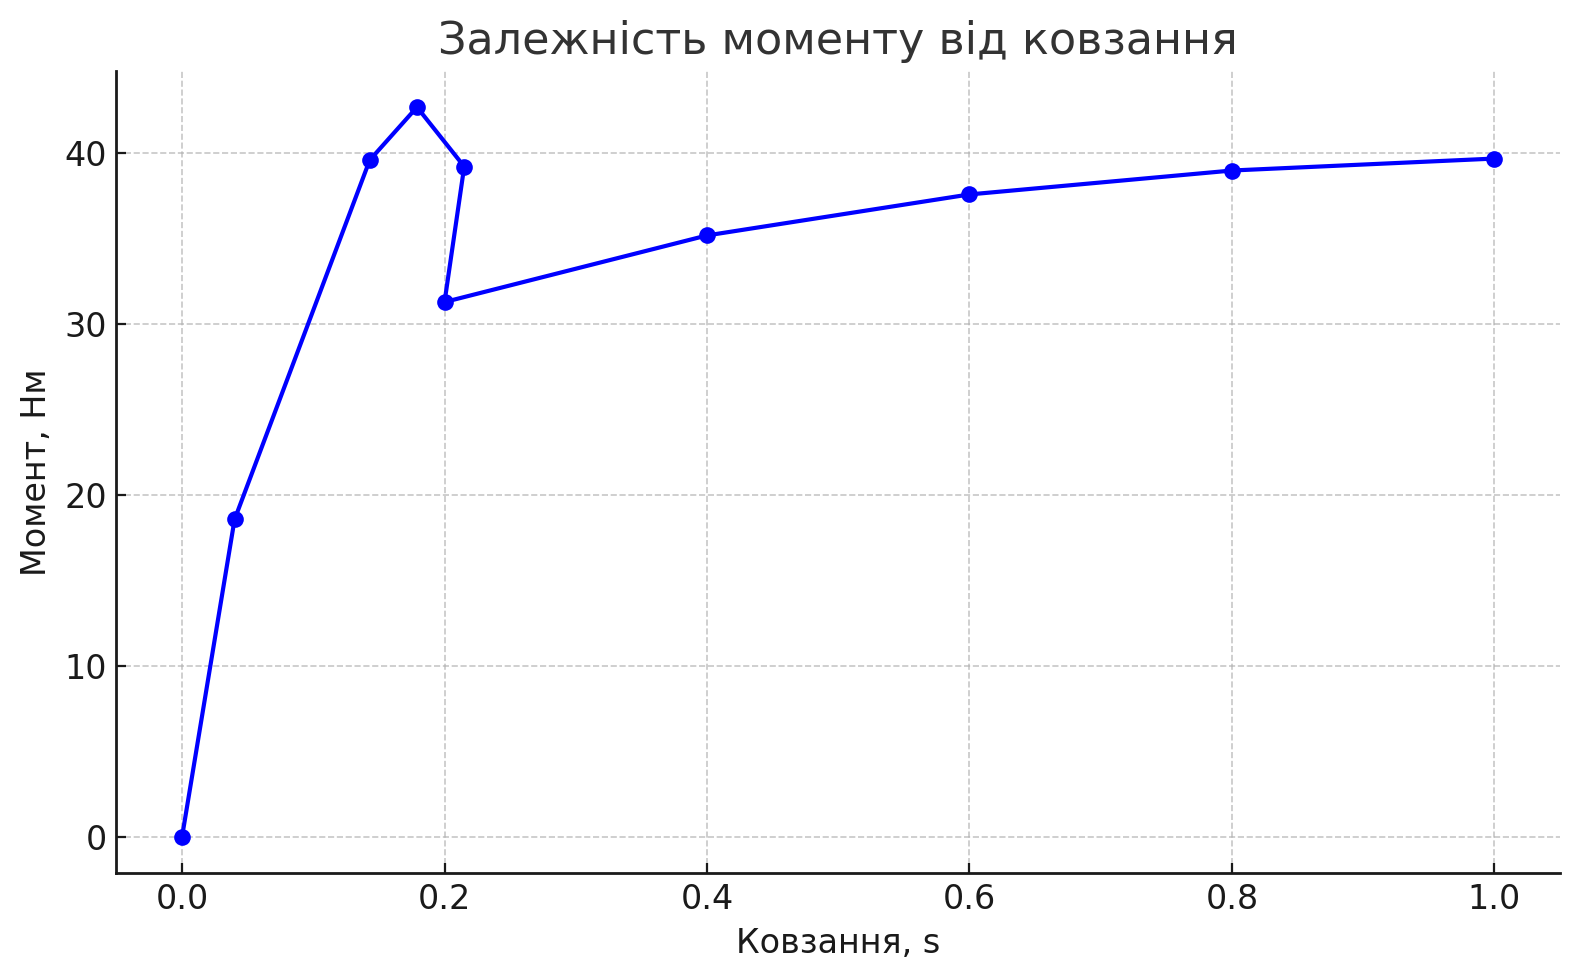
\includegraphics[width=1\textwidth]{imgs/LW2.5.png}
    \caption*{Рис. 2.6: Залежність обертаючого моменту $M$ від ковзання $s$}
\end{figure} 


\section*{Висновки}

Отримані результати дозволяють оцінити параметри роботи трифазного асинхронного двигуна, його енергетичні характеристики та вибір необхідних ємностей для підвищення коефіцієнта потужності.

\section*{Контрольні питання}
\begin{enumerate}
    \item Чому асинхронний двигун так називається? \\
    Асинхронний двигун називається так тому, що частота обертання його ротора не співпадає з частотою обертання магнітного поля статора (яка визначається частотою змінного струму). Різниця між цими частотами називається ковзанням.
    
    \item Чому є небажаною велика сила пускового струму? \\
    Велика сила пускового струму небажана, оскільки вона може призвести до значних механічних та електричних навантажень на двигун і мережу, викликати пошкодження ізоляції проводів, зменшити термін служби обладнання, а також викликати перевантаження трансформаторів і підстанцій.
    
    \item Що використовують для зниження сили пускового струму? \\
    Для зниження сили пускового струму використовують спеціальні пристрої, такі як стартери з обмеженням струму, трансформатори з регульованим напругою або пристрої плавного пуску, що забезпечують поступове збільшення напруги на двигуні.
\end{enumerate}


\end{document}